\begin{figure}[H]
    \centering
    \begin{subfigure}{0.33\textwidth}
        \centering
        \includegraphics[width=0.85\textwidth]{imagens/peppers.png}
        \caption{Original.}
    \end{subfigure}%
    \begin{subfigure}{0.33\textwidth}
        \centering
        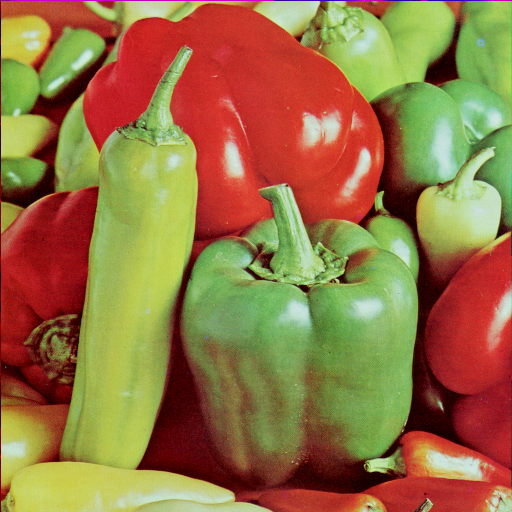
\includegraphics[width=0.85\textwidth]{bits/pep0.png}
        \caption{Ocultação no plano 0.}
    \end{subfigure}
    \begin{subfigure}{0.33\textwidth}
        \centering
        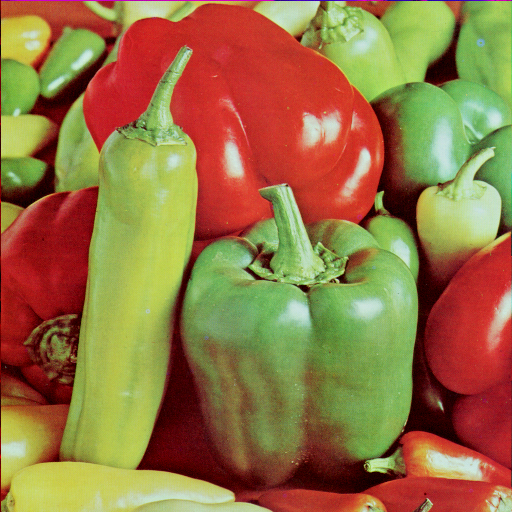
\includegraphics[width=0.85\textwidth]{bits/pep1.png}
        \caption{Ocultação no plano 1.}
    \end{subfigure}\\[8pt]
    \begin{subfigure}{0.33\textwidth}
        \centering
        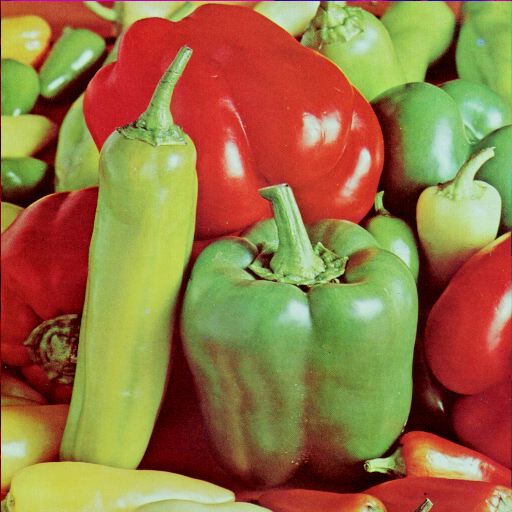
\includegraphics[width=0.85\textwidth]{bits/pep2.png}
        \caption{Ocultação no plano 2.}
    \end{subfigure}%
    \begin{subfigure}{0.33\textwidth}
        \centering
        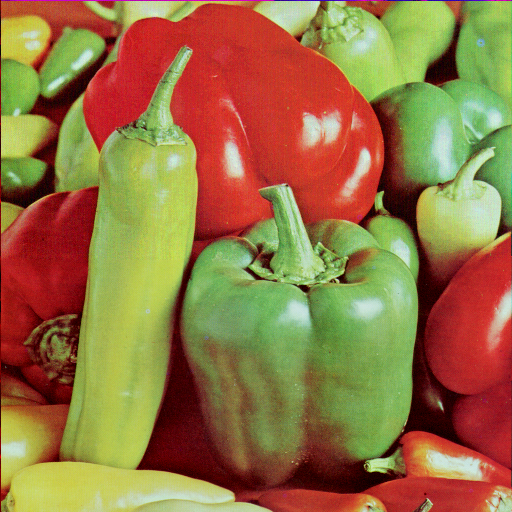
\includegraphics[width=0.85\textwidth]{bits/pep3.png}
        \caption{Ocultação no plano 3.}
    \end{subfigure}%
    \begin{subfigure}{0.33\textwidth}
        \centering
        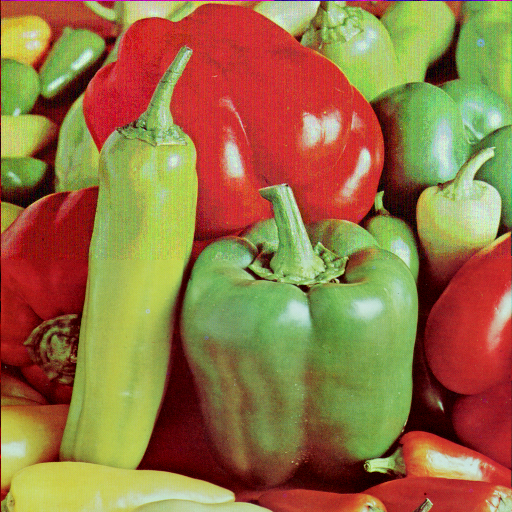
\includegraphics[width=0.85\textwidth]{bits/pep4.png}
        \caption{Ocultação no plano 4.}
    \end{subfigure}

    \caption{Ocultação das primeiras 5 mil linhas de \texttt{words.txt} em \texttt{peppers.png}.}
    \label{fig:peppers}
\end{figure}